\documentclass[12pt]{report}
\usepackage{graphicx}
\usepackage{hyperref}
\usepackage{listings}
\usepackage{xcolor}
\usepackage{pdfpages}

\renewcommand{\bibname}{References}
\title{Shooting Game Architecture with MySQL}

\begin{document}

\includepdf[pages=1]{CoverPage.pdf}

\date{}
\maketitle

\tableofcontents

\chapter{Introduction}

\section{Project Overview}
This project involves integrating a Unity game with a MySQL database. A standard method for creating a game has always been a big challenge faced by game developers. In this project, we aim to create a standard game architecture method for creating a shooting game using Unity as Game Engine and MySQL as backend database for our game.

\section{Keywords}
MySQL, Unity, Odin, Database, Operating System(OS), DBMS, Relational Schema, Conceptual Schema.

\section{Objectives}
\begin{itemize}
    \item Make a standardized shooting game architecture.
    \item Create a MySQL database for our game.
		\item Connect Unity with a MySQL database.
    \item Create a custom editor window to display and manage data inside Unity.
\end{itemize}

\section{Softwares/Frameworks Used}
\begin{itemize}
		\item MySQL.
    \item Unity.
    \item Odin.
    \item Draw.IO.
\end{itemize}

\section{Database Management System}
A Database Management System (DBMS) is a software system that is designed to manage and organize data in a structured manner. It allows users to create, modify, and query a database, as well as manage the security and access controls for that database\cite{geekforgeeks_dbms}.

\subsection{Types of DBMS}
DBMS can be classified into two types: 
Relational Database Management System (RDBMS) and Non-Relational Database Management System (NoSQL or Non-SQL)
\subsection{RDBMS} 
Data is organized in the form of tables and each table has a set of rows and columns. The data are related to each other through primary and foreign keys.
\subsection{NoSQL} 
Data is organized in the form of key-value pairs, documents, graphs, or column-based. These are designed to handle large-scale, high-performance scenarios.

\subsection{MySQL}
MySQL is a fast, easy-to-use RDBMS being used for many small and big businesses. It is developed, marketed and supported by MySQL AB, which is a Swedish company. MySQL is becoming so popular because of many good reasons \cite{tutorialspoint_mysql}.

\begin{itemize}
\item MySQL is released under an open-source license. So you have nothing to pay to use it.
\item MySQL is a very powerful program in its own right. It handles a large subset of the functionality of the most expensive and powerful database packages.
\item MySQL uses a standard form of the well-known SQL data language.
\item MySQL works on many operating systems and with many languages including PHP, PERL, C, C++, JAVA, etc.
\item MySQL works very quickly and works well even with large data sets.
\item MySQL is very friendly to PHP, the most appreciated language for web development.

\item MySQL supports large databases, up to 50 million rows or more in a table. The default file size limit for a table is 4GB, but you can increase this (if your operating system can handle it) to a theoretical limit of 8 million terabytes (TB).

\item MySQL is customizable. The open-source GPL license allows programmers to modify the MySQL software to fit their own specific environments.		
\end{itemize}

\subsection{Database System and DBMS Workflow}
The general workflow of a database system is that queries are passed to a DBMS which interpret it. After succesful execution of a query, OS(Operating System) interacts with actual database and retrieves/add/delete data from database as shown in\ref{fig:db_sys_workflow}. Below is the more refined workflow of a database system. 

Refined Workflow is:
\begin{itemize}
 \item  User/Application → DBMS
 \item DBMS interprets and optimizes the query.
 \item DBMS requests the OS for data access.
 \item OS reads/writes data from/to disk.
 \item OS → DBMS
 \item DBMS processes the data and returns results to User/Application.
\end{itemize}

\begin{figure}[h!]
    \centering
    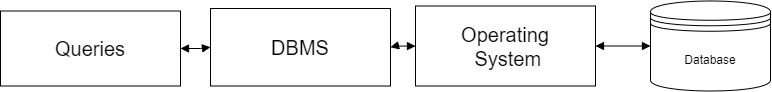
\includegraphics[width=\textwidth]{DBMS_Workflow.png}
    \caption{Database System Workflow}
    \label{fig:db_sys_workflow}
\end{figure}

\section{Unity}
Unity is a cross-platform game engine initially released by Unity Technologies, in 2005. The focus of Unity lies in the development of both 2D and 3D games and interactive content. Unity now supports over 20 different target platforms for deploying, while its most popular platforms are the PC, Android and iOS systems\cite{tutorialspoint_unity}.

Unity features a complete toolkit for designing and building games, including interfaces for graphics, audio, and level-building tools, requiring minimal use of external programs to work on projects.

\subsection{Asset Workflow Overview of Unity}
Importing assets into Unity involves placing files into the Assets folder, which the Unity Editor processes for use in projects. Key steps include adjusting import settings, understanding meta files, and utilizing the Asset Database. After importing, you can create your game by organizing assets into Scenes as GameObjects, scripting interactions, and optimizing downloads using the Addressables system. Building the project involves exporting it to platform-specific binary files and possibly using build automation. Distribution depends on the target platform and can be facilitated by Unity's Cloud Content Delivery service. Finally, the loading process for users is determined by the project's programming and asset bundling strategy, enabling efficient initial downloads and continuous updates\cite{AssetWorkflowUnity}. All this can be seen in figure\ref{fig:AssetWorkflowOverview}.

\begin{figure}[h!]
    \centering
    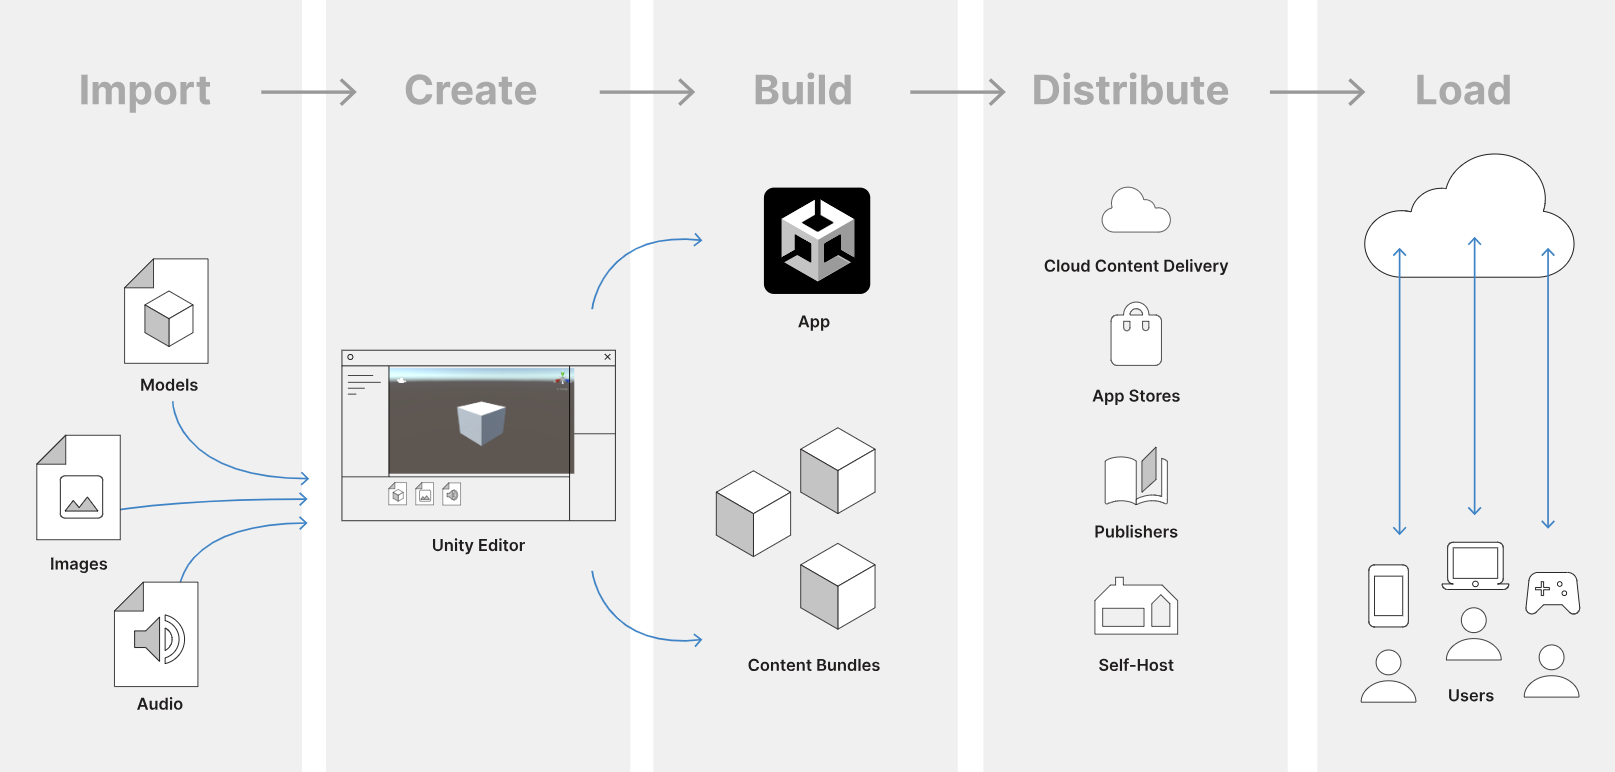
\includegraphics[width=\textwidth]{AssetWorkflowUnity.png}
    \caption{Asset Workflow Overview}
    \label{fig:AssetWorkflowOverview}
\end{figure}

\section{Odin}
Odin Inspector is a plugin for Unity that lets you enjoy all the workflow benefits of having a powerful, customized and user-friendly editor, without ever having to write a single line of custom editor code.
Instead of writing and maintaining thousands of lines of custom editor code, developers can annotate their data structures with our 100+ building block attributes to quickly and easily build user-friendly editors for their entire team.
Odin is additionally packed to the brim with a broad suite of editor utilities for many common tasks like creating custom editor windows and much, much more\cite{odininspector}.

\section{Draw.IO}
draw.io, also known as Diagrams.net, is a customized tool for creating diagrams and charts. It offers existing automated layout options, or the user can design a custom layout for their preferences. The tool provides a wide range of shapes and hundreds of graphic components to let you create unique diagrams. Depending on your needs, draw.io can keep saved charts in the cloud or in network storage at a data center. It works both offline and on mobile devices. The service does not keep any of your data or claim ownership of your creations, ensuring that you are safe regardless of where or how you work\cite{drawio_ref}.

\subsection{Role of Draw.IO in this project}
In this project, draw.io is used for making diagrams for conceptual and relational schema. Draw.io is a great tool and saves a lot of time when making a schema for a database.

\chapter{Logical Database Design}

\section{Business Rules}
Following business rules were followed during the database design.

\begin{itemize}
    \item A player can participate in multiple quests.
		\item A player can achieve multiple achievements.
		\item Stores contain multiple characters and weapons..
    \item Characters are associated with a store and have a price.
  	\item Each quest can be assigned to multiple players.
	  \item Each quest provides a reward and has a specific type.
		\item A player can play one or many levels.
    \item Each level can have multiple associated bosses and items.
    \item A player can unlock multiple achievements.
		\item The Unlock Achievement Certificate table tracks which achievements have been unlocked by which players.		
		\item Bosses are associated with a specific level and each boss has unique abilities.
		\item Items can be classified as different types (e.g., Enemy AI, Checkpoint, Pickup).
		
\end{itemize}

\section{Conceptual Schema}
The database schema includes tables for players, quests, characters, stores, and other game entities. The schema is designed to handle various relationships between these entities. 

\begin{figure}[h!]
    \centering
    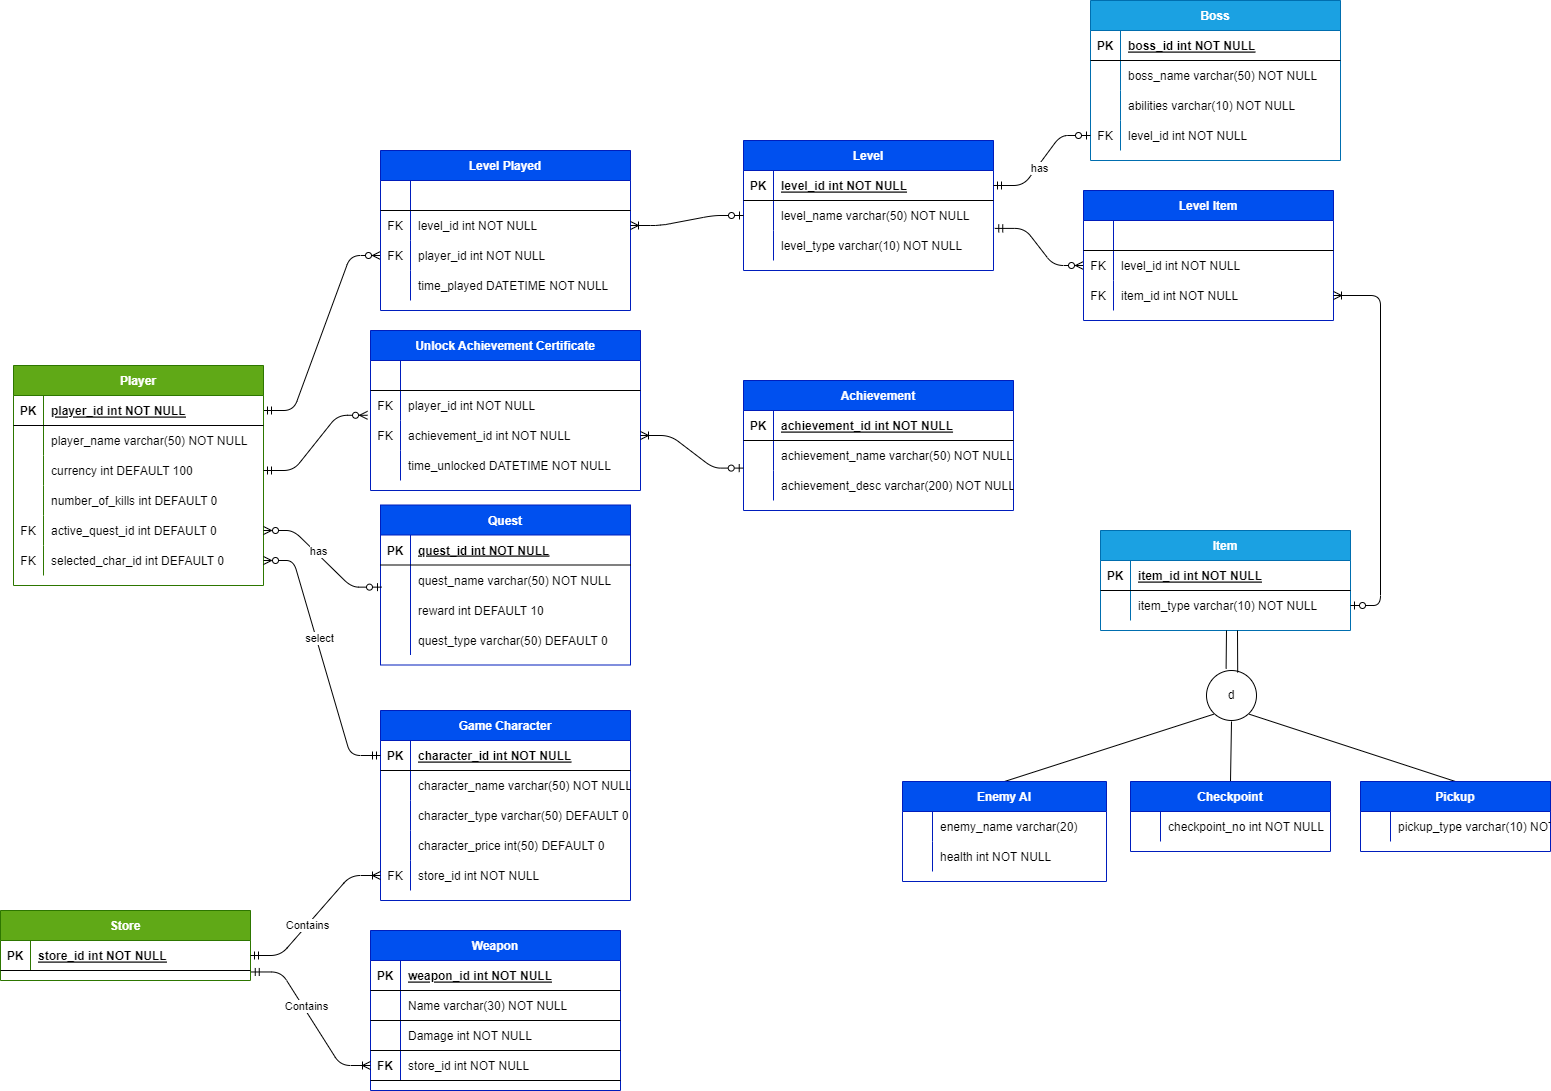
\includegraphics[width=\textwidth]{database_schema.png}
    \caption{Database Conceptual Schema}
    \label{fig:db_schema}
\end{figure}

\section{Relational Schema}
The following normalized relational schema is obtained from the conceptual schema from previous section.

\subsection{Relational Schema Sketch}
Sketch of Relational Schema is given below.
\begin{figure}[h!]
    \centering
    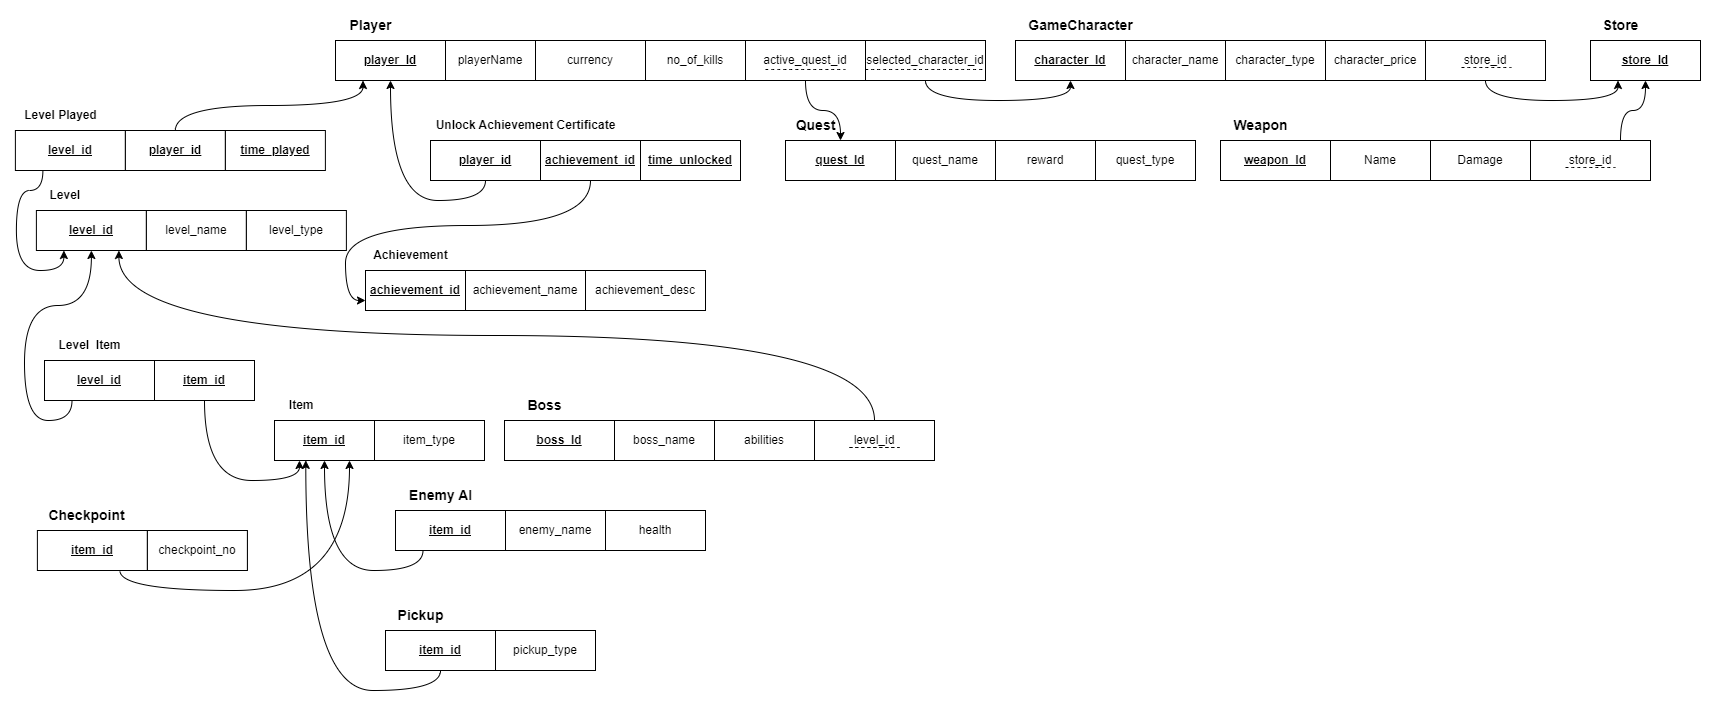
\includegraphics[width=\textwidth]{relational_schema.png}
    \caption{Database Relational Schema}
    \label{fig:db_relational_schema}
\end{figure}

%\subsection{Table Names}
%\begin{itemize}
% \item achievement                    
% \item boss                           
% \item checkpoint                     
% \item enemyAi                       
% \item gamecharacter                 
% \item item                           
% \item level                           
% \item levelItem
% \item levelPlayed                   
% \item pickup                         
% \item player                         
% \item quest                          
% \item store                          
% \item unlockAchievementCertificate 
% \item weapon
%\end{itemize}

\chapter{Physical Database Design}

\section{Physical Database Structure}
After running successful SQL queries, following tables we created in the database. These tables are physically stored in the memory of the computer as shown in\ref{fig:db_sys_workflow}.

\begin{figure}[h!]
    \centering
    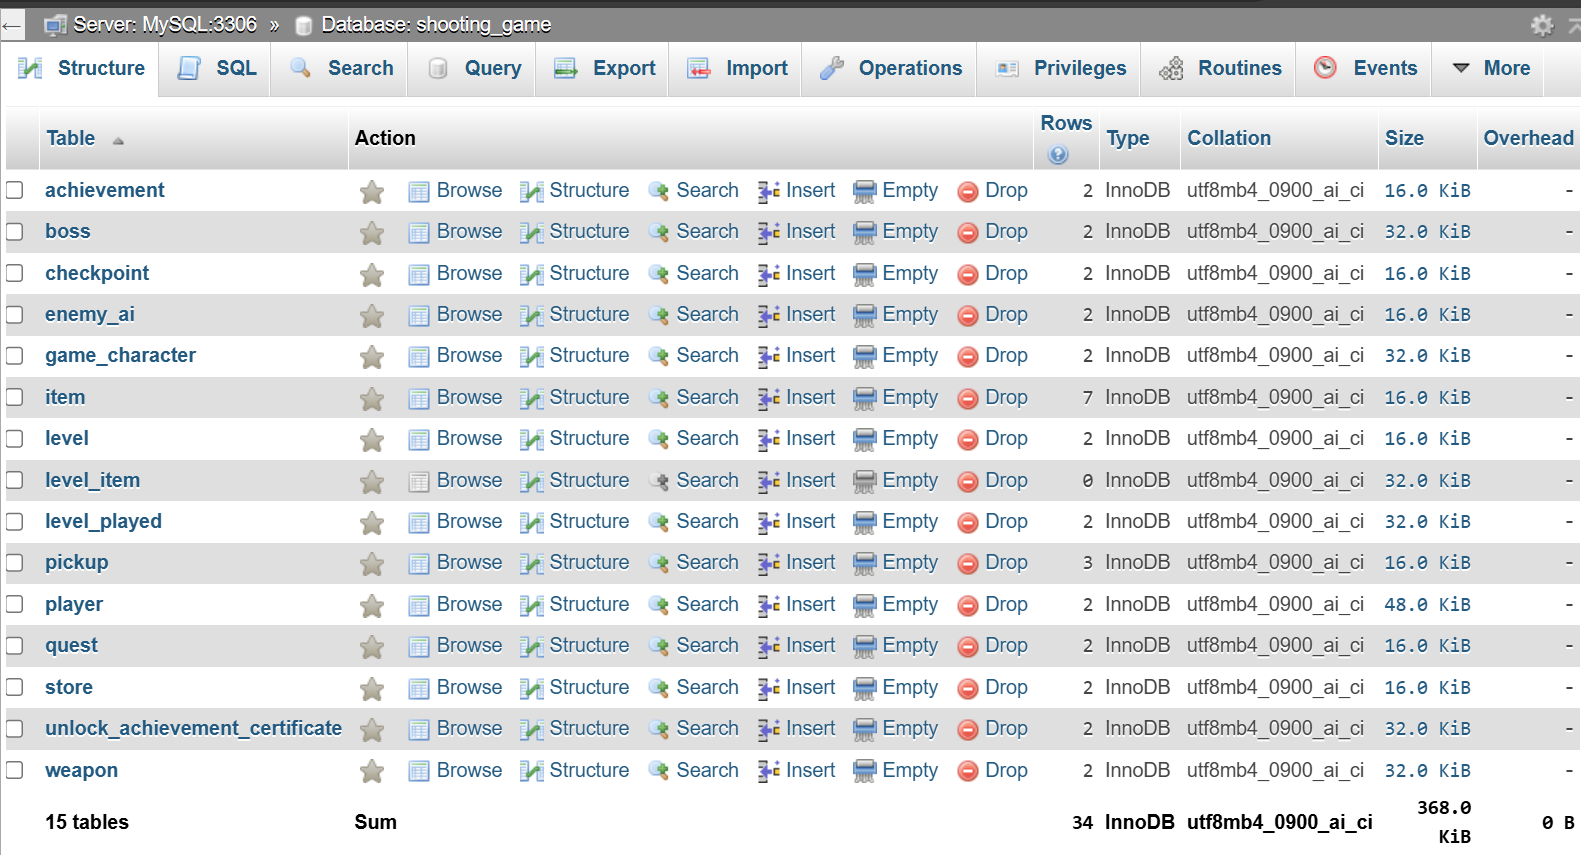
\includegraphics[width=\textwidth]{db_physical_structure.png}
    \caption{Database Physical Structure}
    \label{fig:db_physical_structure}
\end{figure}

\section{SQL Queries for Tables Creation}
Following queries were given to MySQL for tables creation.

\subsection{Achievement}
\begin{verbatim}
CREATE TABLE achievement(
  `achievement_id` int NOT NULL,
  `achievement_name` varchar(50) NOT NULL,
  `achievement_desc` varchar(200) NOT NULL,
  PRIMARY KEY (`achievement_id`));

\end{verbatim}

\subsection{Boss}
\begin{verbatim}
CREATE TABLE boss(
  `boss_id` int NOT NULL,
  `boss_name` varchar(50) NOT NULL,
  `abilities` varchar(50) NOT NULL,
  `level_id` int NOT NULL,
  PRIMARY KEY (`boss_id`),
  KEY `level_id` (`level_id`));

\end{verbatim}
\subsection{Checkpoint}
\begin{verbatim}
CREATE TABLE checkpoint(
  `item_id` int NOT NULL,
  `checkpoint_no` int NOT NULL,
  PRIMARY KEY (`item_id`));

\end{verbatim}
\subsection{Enemy AI}
\begin{verbatim}
CREATE TABLE enemy_ai(
  `item_id` int NOT NULL,
  `health` int NOT NULL,
  `enemy_name` varchar(20) DEFAULT NULL,
  PRIMARY KEY (`item_id`));
\end{verbatim}

\subsection{Game Character}
\begin{verbatim}
CREATE TABLE game_character(
  `character_id` int NOT NULL,
  `character_name` varchar(50) NOT NULL,
  `character_type` varchar(50) DEFAULT NULL,
  `character_price` int DEFAULT '0',
  `store_id` int NOT NULL,
  PRIMARY KEY (`character_id`),
  KEY `store_id` (`store_id`));
\end{verbatim}

\subsection{Item}
\begin{verbatim}
CREATE TABLE item(
  `item_id` int NOT NULL,
  `item_type` varchar(10) NOT NULL,
  PRIMARY KEY (`item_id`));
\end{verbatim}

\subsection{Level}
\begin{verbatim}
CREATE TABLE level(
  `level_id` int NOT NULL,
  `level_name` varchar(50) NOT NULL,
  `level_type` varchar(10) NOT NULL,
  PRIMARY KEY (`level_id`));
\end{verbatim}

\subsection{Level Item}
\begin{verbatim}
CREATE TABLE level_item(
  `level_id` int NOT NULL,
  `item_id` int NOT NULL,
  PRIMARY KEY (`level_id`,`item_id`),
  KEY `item_id` (`item_id`));
\end{verbatim}

\subsection{Level Played}
\begin{verbatim}
CREATE TABLE level_played(
  `level_id` int NOT NULL,
  `player_id` int NOT NULL,
  `time_played` datetime DEFAULT NULL,
  PRIMARY KEY (`level_id`,`player_id`),
  KEY `player_id` (`player_id`));
\end{verbatim}

\subsection{Pickup}
\begin{verbatim}
CREATE TABLE pickup(
  `item_id` int NOT NULL,
  `pickup_type` varchar(20) DEFAULT NULL,
  PRIMARY KEY (`item_id`));
\end{verbatim}

\subsection{Player}
\begin{verbatim}
CREATE TABLE player(
  `player_id` int NOT NULL,
  `player_name` varchar(50) NOT NULL,
  `currency` int DEFAULT '100',
  `number_of_kills` int DEFAULT '0',
  `active_quest_id` int DEFAULT '0',
  `selected_char_id` int DEFAULT '0',
  PRIMARY KEY (`player_id`),
  KEY `active_quest_id` (`active_quest_id`),
  KEY `selected_char_id` (`selected_char_id`));
\end{verbatim}
\subsection{Quest}
\begin{verbatim}
CREATE TABLE quest(
  `quest_id` int NOT NULL,
  `quest_name` varchar(50) NOT NULL,
  `reward` int DEFAULT '10',
  `quest_type` varchar(50) DEFAULT '0',
  PRIMARY KEY (`quest_id`));

\end{verbatim}
\subsection{Store}
\begin{verbatim}
CREATE TABLE store(
  `store_id` int NOT NULL,
  PRIMARY KEY (`store_id`));

\end{verbatim}
\subsection{Unlock Achievement Certificate}
\begin{verbatim}
CREATE TABLE unlock_achievement_certificate(
  `player_id` int NOT NULL,
  `achievement_id` int NOT NULL,
  `time_unlocked` datetime DEFAULT NULL,
  PRIMARY KEY (`player_id`,`achievement_id`),
  KEY `achievement_id` (`achievement_id`));
\end{verbatim}

\subsection{Weapon}
\begin{verbatim}
CREATE TABLE weapon(
  `weapon_id` int NOT NULL,
  `name` varchar(30) NOT NULL,
  `damage` int NOT NULL,
  `store_id` int DEFAULT NULL,
  PRIMARY KEY (`weapon_id`),
  KEY `store_id` (`store_id`));
\end{verbatim}

\chapter{Integrating MySQL with Unity}

\section{Introduction}
Integrating MySQL with Unity can provide robust backend support for multiplayer games, persistent data storage, and complex data queries. MySQL Connector/NET, a data provider for MySQL, enables Unity to communicate with MySQL databases.

\section{Setting Up MySQL Connector/NET in Unity}
\begin{itemize}
 \item First of all, Download MySQL Connector/NET                    
 \item Download and install the appropriate version for your system.    
 \item Add MySQL.Data.dll to Unity.    
 \item Locate the MySql.Data.dll file from the installation directory (usually found in the assemblies or lib directory of the MySQL Connector installation).    
 \item Copy MySql.Data.dll to the Assets/Plugins folder in your Unity project as shown in figure\ref{fig:unity_plugins}.   
\end{itemize}       
\begin{figure}[h!]
    \centering
    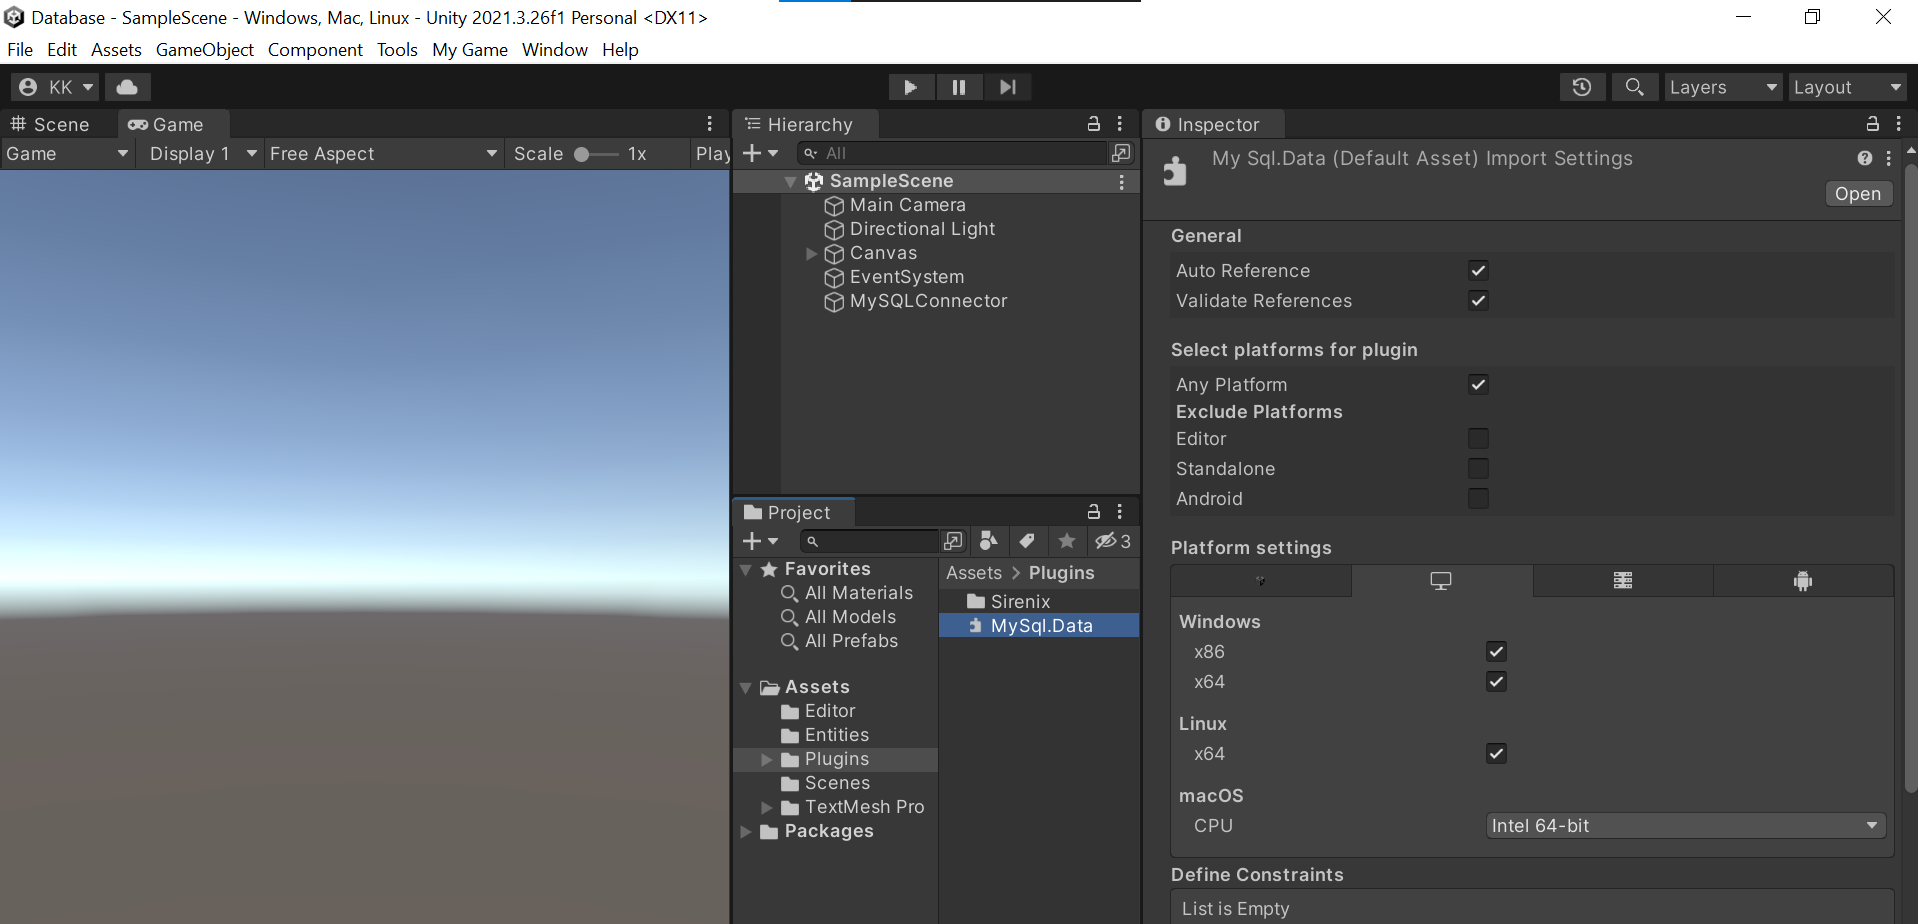
\includegraphics[width=\textwidth]{unity_plugins.png}
    \caption{MySql.Data.dll in Unity Plugins Folder for connecting MySQL with Unity}
    \label{fig:unity_plugins}
\end{figure}

\section{Database Connection Code - MySQLDatabase class}
The code shown in figure\ref{fig:unity_db_connector_code1} shows how can we establish connection with MySQL from Unity c# class. The database credentials are given in the string argument of the constructor.

\begin{figure}[h!]
    \centering
    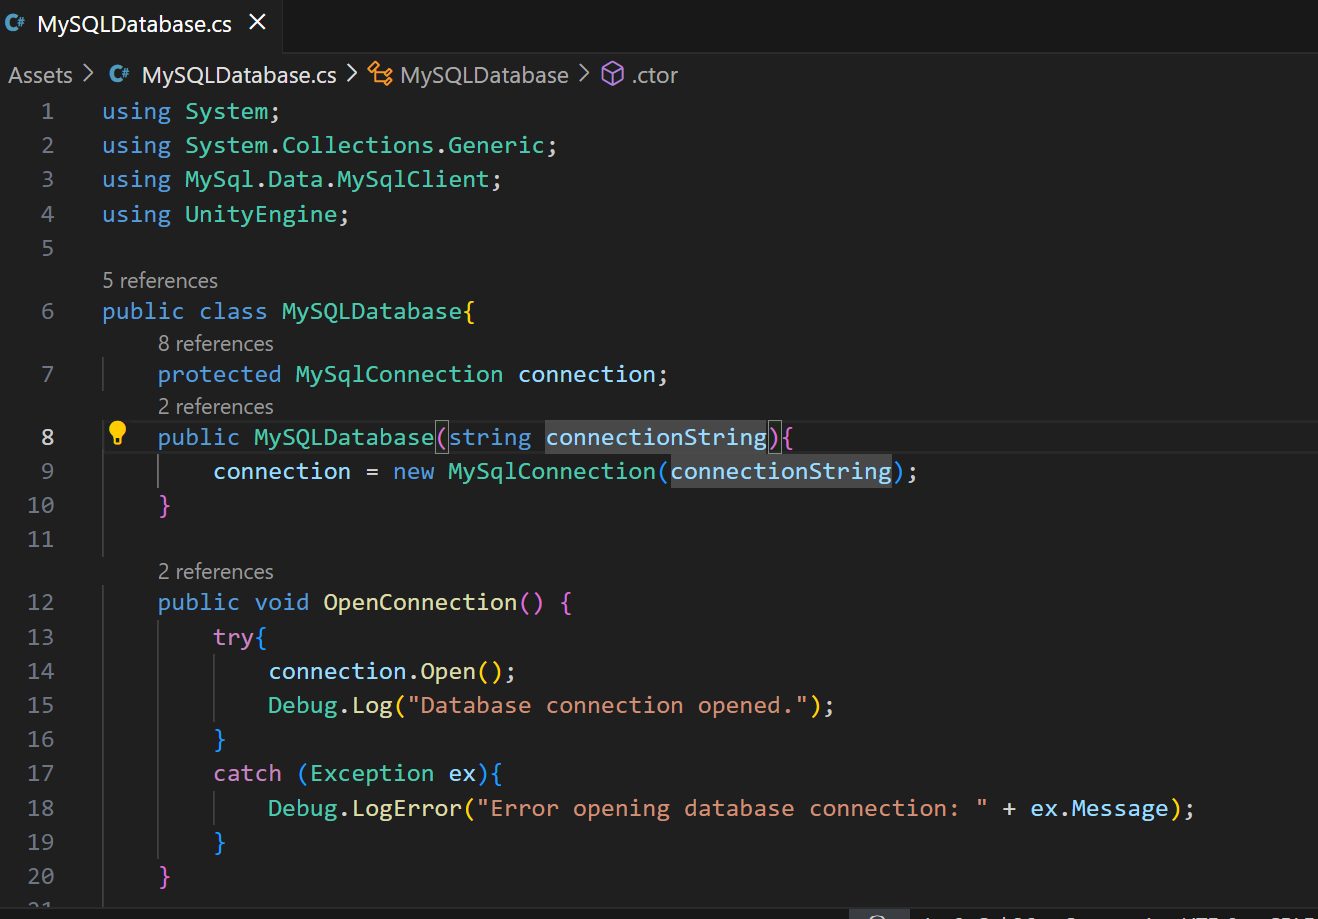
\includegraphics[width=\textwidth]{unity_database_connector_code1.png}
    \caption{Database Connection Code - MySQLDatabase class}
    \label{fig:unity_db_connector_code1}
\end{figure}

\section{Serializing and displaying the data}
This is the last part of the implementation phase. In order to get data and show it in Unity\cite{serialization}, We have created a C# class for each table. This class serializes the data and this data is shown on the editor window of Unity. Figure \ref{fig:player_class_code} Shows the code of Player class. 

\begin{figure}[h!]
    \centering
    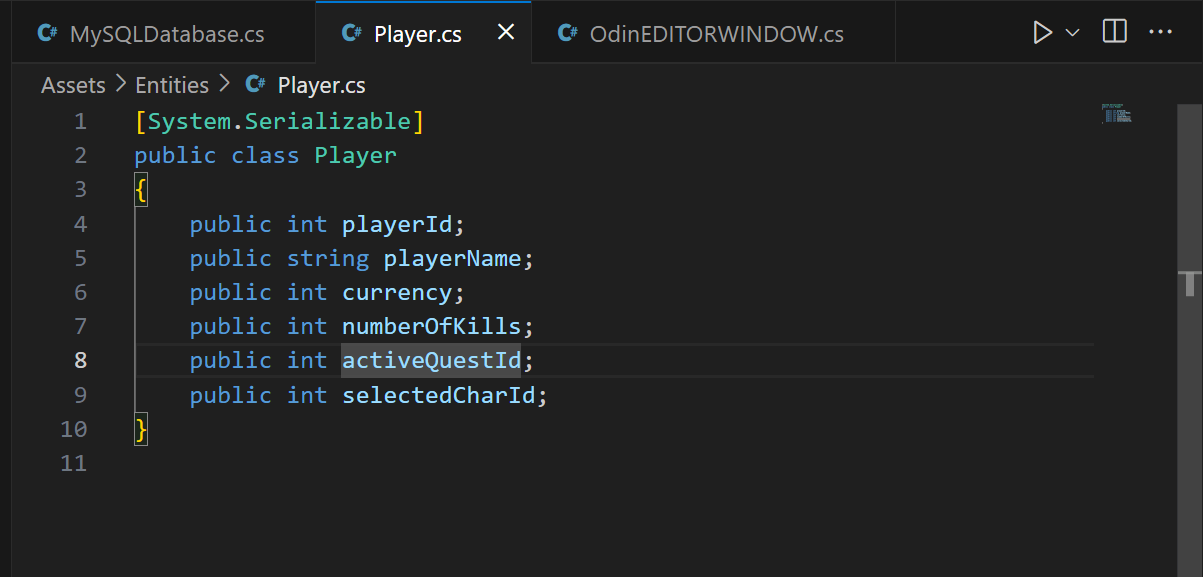
\includegraphics[width=\textwidth]{player_class_code.png}
    \caption{Player class code for data serialization}
    \label{fig:player_class_code}
\end{figure}

\section{Role of Odin}
Odin is a great tool for making Editor Windows and Serializing data in Unity. The following script demonstrate the use of Odin Library and MySQLDatabase class to get data from MySQL and show it on Unity Editor  

\begin{figure}[h!]
    \centering
    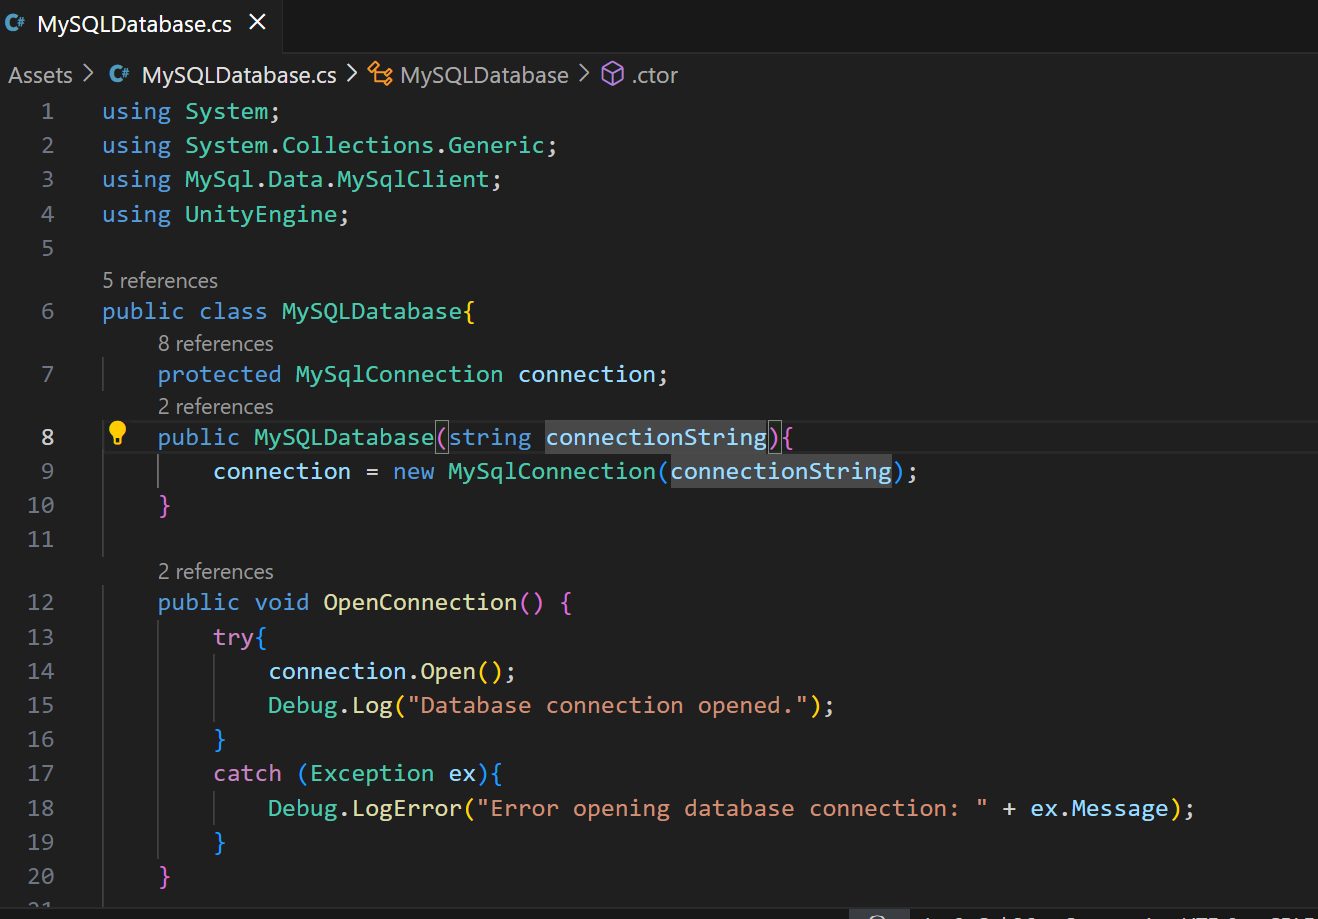
\includegraphics[width=\textwidth]{unity_database_connector_code1.png}
    \caption{Database Connection Code - MySQLDatabase class}
    \label{fig:unity_db_connector_code1}
\end{figure}

\chapter{Conclusion}
This project demonstrates how to integrate a Unity game with a MySQL database. The custom editor window provides an easy way to display and manage the data within the Unity Editor.

\section{Final Output}
Following are some of the snapshots of the output of this project.

\begin{figure}[h!]
    \centering
    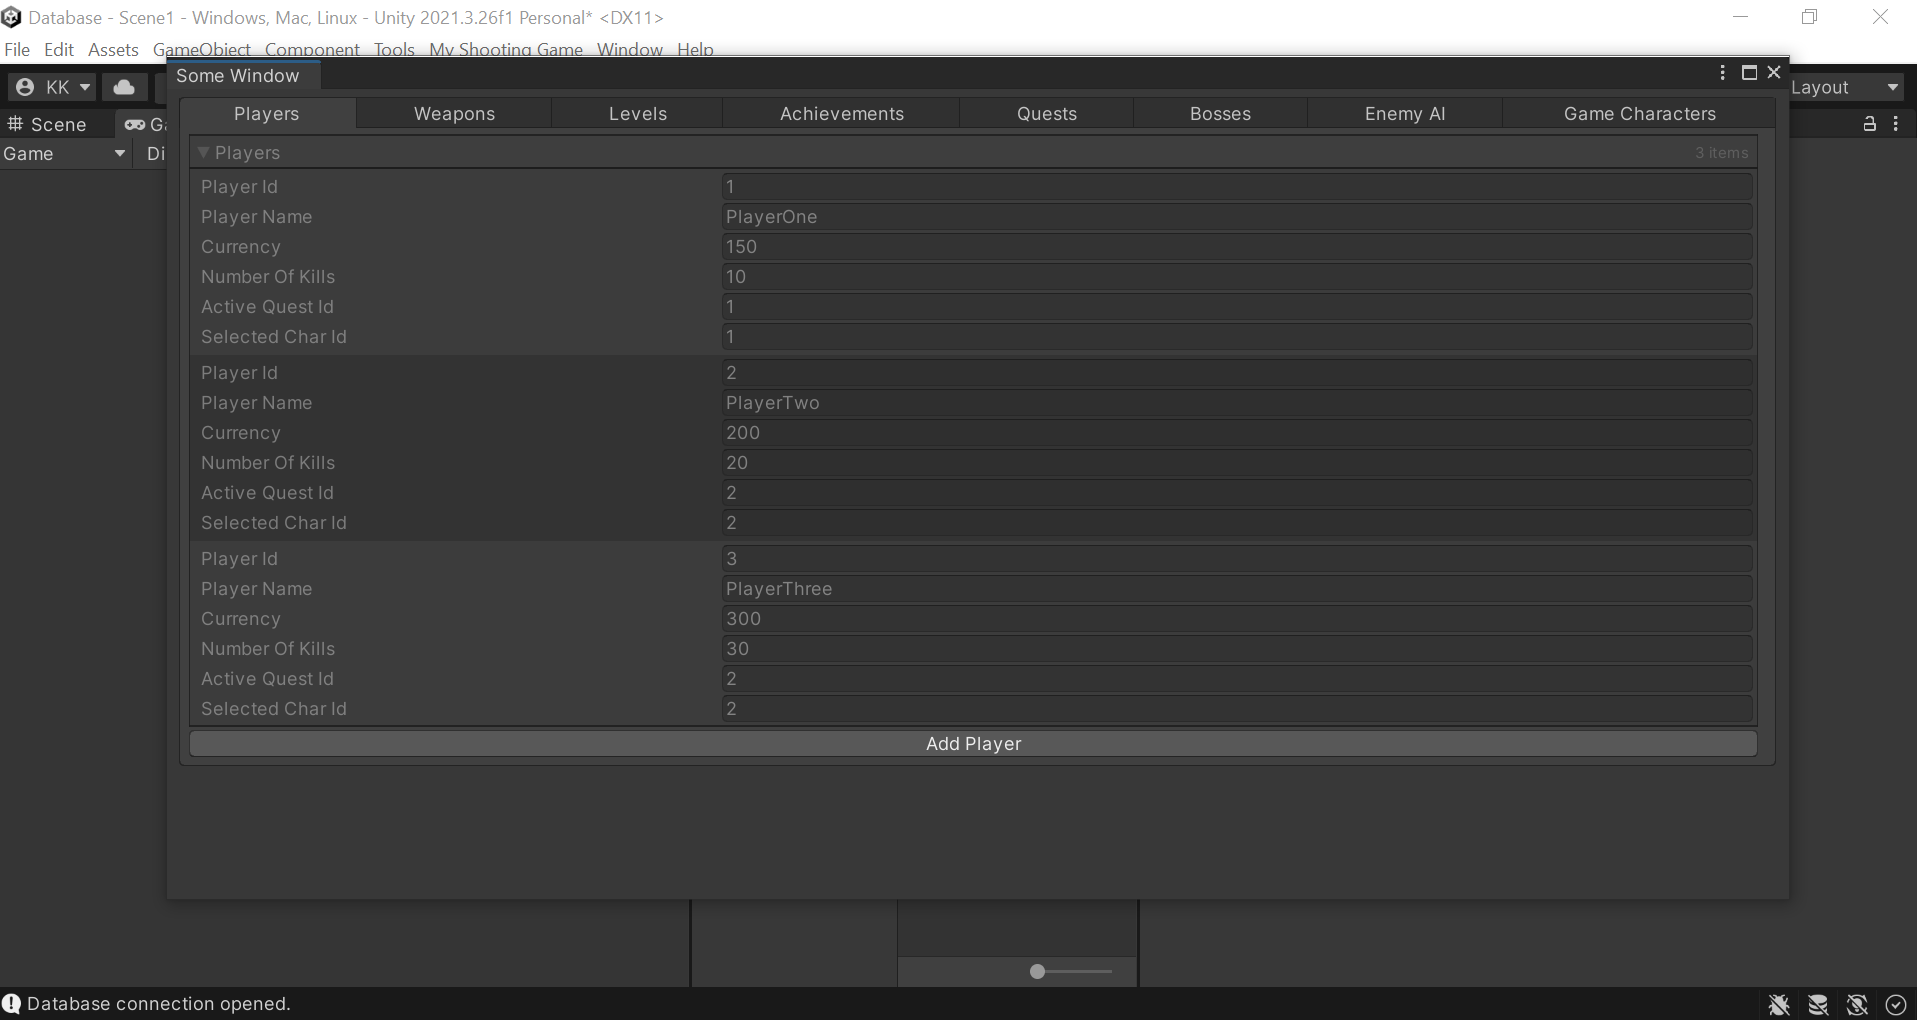
\includegraphics[width=\textwidth]{Output1.png}
    \caption{Output Snapshot 1}
    \label{fig:Output1}
\end{figure}
\begin{figure}[h!]
    \centering
    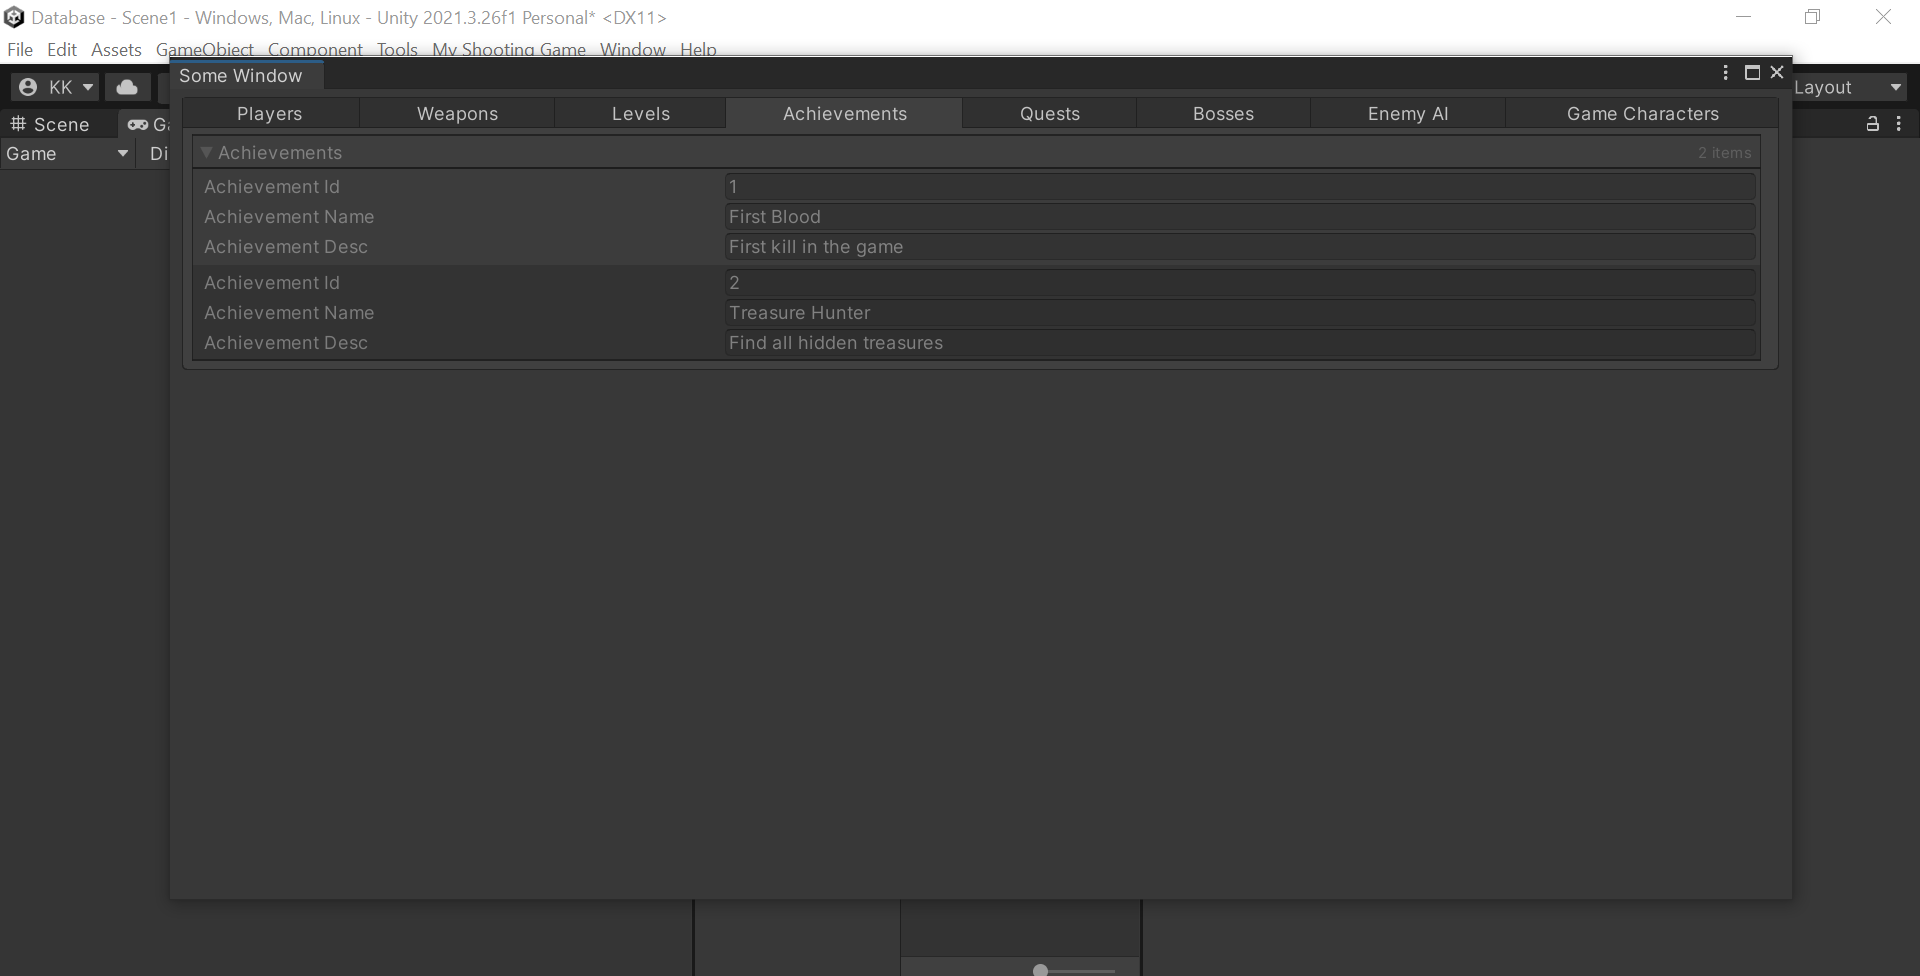
\includegraphics[width=\textwidth]{Output2.png}
    \caption{Output Snapshot 2}
    \label{fig:Output2}
\end{figure}

\section{Future Work}
Future work could include enhancing the database operations, adding more features to the custom editor window, and optimizing the performance of the database interactions.

\begin{thebibliography}{9}

\bibitem{tutorialspoint_mysql}
https://www.tutorialspoint.com/mysql/mysql-introduction.htm

\bibitem{geekforgeeks_dbms}
https://www.geeksforgeeks.org/introduction-of-dbms-database-management-system-set-1

\bibitem{AssetWorkflowUnity}
https://docs.unity3d.com/Manual/AssetWorkflow.html

\bibitem{tutorialspoint_unity}
https://www.tutorialspoint.com/unity/unity_introduction.htm

\bibitem{odininspector}
https://odininspector.com

\bibitem{serialization}
https://docs.unity3d.com/Manual/script-Serialization.html

\bibitem{drawio_ref}
https://medium.com/@hasaliedirisinghe/user-guide-to-draw-io-6a1a4d7b5d33
\end{thebibliography}
\end{document}
